\achapter{18}{Connected Spaces}\label{sec:Connected_topology}


\vspace*{-17 pt}
\framebox{
\parbox{\dimexpr\linewidth-3\fboxsep-3\fboxrule}
{\begin{fqs}
\item What is a connected subset of a topological space?
\item What is a separation of a subset of a topological space? Why are separations useful?
\item What are the connected subsets of $\R$?
\item What is a connected component of a topological space?
\item What is an application of connectedness?
\item What is a cut set of a topological space? Why are cut sets useful?
\end{fqs}}}

\vspace*{13 pt}

\csection{Introduction}

The term ``connected" should bring up images of something that is one piece, not separated. There is more than one way we can interpret the notion of connectedness in topological spaces. For example, we might consider a topological space to be connected if we can't separate it into disjoint pieces in any non-trivial way. As another possibility, we might consider a topological space to be connected if there is always a path from one point in the spaced to another, provided we define what ``path' means. These are different notions of connectedness, and we focus on the first notion in this section.

Connectedness is an important property, and one that we encounter in the calculus. For example, we will see in this section that the Intermediate Value Theorem relies on connected subsets of $\R$. To define a connected set, we will need to have a way to understand when and how a set can be separated into different pieces. Since a topology is defined by open sets, when we want to separate objects we will do so with open sets. This is similar to the idea behind Hausdorff spaces, except that we now want to know if a set can be separated in some way rather than separating points.

As an example to motivate the definition, consider the sets $X = (0,1) \cup (1,2)$ and $Y = [1,2]$ in $\R$ with the Euclidean topology. Notice that we can write $X$ as the union of two disjoint open sets $X_1 = (0,1)$ and $X_2 = (1,2)$. So we shouldn't think of $X$ as being connected. However, if we attempt to write $Y$ as a union of two subsets, say $Y_1 = [1,1.5)$ and $Y_2 = [1.5,2]$, it is impossible for both of these subsets to be open and disjoint. So $Y$ is a set we should consider to be connected. This is the notion of connectedness that we wish to investigate. 

\begin{definition}  A topological space $(X,\tau)$ is \textbf{connected}\index{connected space} if $X$ cannot be written as the union of two disjoint, nonempty, open subsets. A subset $A$ of a topological space topological space $(X,\tau)$ is connected if $A$ is connected in the subspace topology. 
\end{definition}

%\begin{definition}  A subset $A$ of a topological space $(X,\tau)$ is \textbf{connected}\index{connected space} if $A$ cannot be written as the union of two disjoint, nonempty, relatively open subsets in the subspace topology. A topological space $X$ is connected if $X$ is a connected subset of $X$.
%\end{definition}

If a set $X$ is not connected, we say that $X$ is disconnected. If $X$ is a disconnected topological space, then there exist disjoint nonempty open sets $U$ and $V$ such that $X = U \cup V$. %Such a pair of sets $U$ and $V$ is called a \emph{separation}\index{separation} of $X$. 

\begin{pa} Can the subset $A$ of the topological space $X$ be written as the union of two disjoint nonempty relatively open sets?
\be
\item The set $A = \{a, b\}$ in $(X, \tau)$ with $X = \{a, b, c, d\}$ and $\tau = \{\emptyset, \{a\}, \{b\}, \{a, b\}, X\}$.

\item The set $A = \{a, b, c\}$ in $(X, \tau)$ with $X = \{a,b,c,d,e,f\}$ and 
\[\tau = \{\emptyset, \{a\}, \{c,d\}, \{a, c, d\}, \{b,c,d,e,f\}, X\}.\]

\item  The set $A = X$ with $X = \{a,b,c,d\}$ and 
\[\tau = \{\emptyset, \{b\}, \{c\}, \{a,b\}, \{b,c\}, \{a,b,c\}, \{b,c,d\}, X\}.\]

\item The set $A = \{d, f\}$ in $X = \{a, b, c, d, e, f\}$ with the discrete topology. Generalize your findings.

\item The set $A = \{a, c, d\}$ in $X = \{a, b, c, d, e\}$ with the indiscrete topology. Generalize your findings.

\item The set $A = \Z$ in $X = \R$ with the finite complement topology. Generalize your findings.

\item The set $A = X$ in $X = \{x \in \R \ \mid \ 1 \leq x \leq 2 \text{ or }  3 < x < 4\}$ with the subspace metric topology from $(\R, d_E)$.

\item The set $A = X$ in $X = \left\{(x, y) \in \R^2 \ \mid \  y = \frac{1}{x} \text{ or } y = 0\right\}$ with open sets 
\[\tau = \{U  \cap X \ \mid \ U \text{ is open in the Euclidean Topology on } \R^2\}.\]

\ee

\end{pa}

\begin{comment}

\ActivitySolution

\be
\item The answer is yes. Note that $A = \{a\} \cup \{b\}$, where $\{a\} = A \cap \{a\}$ and $\{b\} = A \cap \{b\}$ are relatively open sets.

\item  The answer is yes. Both $\{a\} = A \cap \{a\}$ and $\{b, c\} = A \cap  \{b, c, d, e, f\}$ are relatively open sets and $A = \{a\} \cup \{b, c\}$.

\item  The answer is no. The only disjoint open sets of $X$ are $\{b\}$ and $\{c\}$ and their union is not $X$. 

\item  The answer is yes. Since every subset of $X$ is open, we can write $A$ as a disjoint union of the open sets $\{d\}$ and $\{f\}$. This argument can be applied to any subset of $X$ containing two or more elements. To see why, let $(X, \tau)$ be a topological space where $\tau$ is the discrete topology, and let $A$ be a subset of $X$ with two or more elements. Let $a \in A$ and let $O = \cup_{\substack{x \in A}\\{x \neq a}}$. Note that $O$ is open and $A$ is the disjoint union of $\{a\}$ with $O$.

\item  The are no proper open sets in $X$, so no proper relatively open sets. Thus, $A$ cannot be written as a disjoint union of nonempty proper open sets. This applies to any space with the indiscrete topology.

\item We have seen that the subspace topology of an infinite subset of a topological space with the finite complement topology is the finite complement topology. Let $U$ and $V$ be relatively open sets in $\Z$. Then $\Z \setminus (U \cap V )$ is a finite set. This means that $U \cap V$ is an infinite set. So either $U$ is infinite or $V$ is infinite, and there are no disjoint relatively open sets in $\Z$. Thus $\Z$ cannot be written as a disjoint union of nonempty proper open sets.

Recall that if $X$ is a finite set, the finite complement topology on $X$ is just the discrete topology. We discussed the discrete topology in problem 3. If $X$ is an infinite set with the finite complement topology, then the same argument as above shows that no subset of $X$ can be written as a disjoint union of nonempty proper relatively open sets.

\item Notice that $[1, 2] = (0, 2.5) \cap X$ and $(3, 4) = (3, 4) \cap X$, so both $[1, 2]$ and $(3, 4)$ are open in $X$. Then $X$ can be written as a disjoint union of nonempty proper open sets as $X = [1, 2] \cup (3, 4)$.

\begin{figure}[h]
\begin{center}
\resizebox{!}{2.5in}{\includegraphics{PA_18_1.eps}}
\caption{The set $O$.} 
\label{F:PA_18_1}
\end{center}
\end{figure}

\item  Let $Q_1 = \{(x, y) \ \mid| \  x > 0 \text{ and } y > 0\}$ and let $Q_4 = \{(x, y) \ \mid| \  x < 0 \text{ and } y < 0\}$. Then $Q_1$ and $Q_4$ are open sets in $\R^2$, so $O_1 = Q_1 \cap A$ and $O_2 = Q_4 \cap A$ are relatively open in $A$. Note that $O_1$ is the portion of the graph of $y = \frac{1}{x}$ in the first quadrant and $O_2$ is the portion of the graph of $y = \frac{1}{x}$ in the fourth quadrant. Now let 
\[O = \left\{(x,y) \mid |x| < 1 \text{ and } |y| < \frac{1}{4}, |x| \geq 1 \text{ and } y < \frac{1}{x^2}\right\}\]
as illustrated in Figure \ref{F:PA_18_1}. Note that $O \cap A$ is the line $y=0$. 

Now let $U = O_1 \cup O_2$ and $V = O \cap A$. Then $U$ and $V$ are nonempty open sets in $A$. Since all of the points in $V$ satisfy $y = 0$ and none of the points in $U$ have $y = 0$, we see that $U \cap V = \emptyset$. So $A$ is disconnected.


\ee

\end{comment}


\csection{Connected Sets}

As we learned in our preview activity, connected sets are those sets that cannot be separated into a union of disjoint open sets. Another characterization of connectedness is established in the next activity.

\begin{activity} Let $(X, \tau)$ be a topological space.
\ba
\item Assume that $X$ is a connected space, and let $A$ be a subset of $X$ that is both open and closed. What happens if we combine $A$ and $X \setminus A$? What does the fact that $X$ is connected tell us about $A$?  

\item Now assume that the only subsets of $X$ that are both open and closed are $\emptyset$ and $X$. Must it follow that $X$ is connected? Prove your assertion. 

\item Summarize the result of this activity into a theorem of the form ``A topological space $(X, \tau)$ is connected if and only if ... ".

\ea
\end{activity} 

\begin{comment}

\ActivitySolution

\ba
\item The set $X = A \cup (X \setminus A)$ expresses $X$ as a disjoint union of two subsets. Since $X$ is connected, $A$ cannot be a proper subset of $X$, so $A = \emptyset$ or $A = X$.

\item Suppose that $A$ and $B$ are disjoint open subsets of $X$ such that $X = A \cup B$. It follows that $B = X \setminus A$ and so $A$ is closed. Since $A$ is both open and closed, we can conclude that $A = \emptyset$ or $A = X$. This implies that there are no proper disjoint open subsets of $X$ whose union is $X$. Therefore, $X$ is connected. 

\item The appropriate theorem is

\noindent \textbf{Theorem.} A topological space $(X, \tau)$ is connected if and only if the only sets that are both open and closed in $X$ are $\emptyset$ and $X$. 

\ea

\end{comment}

A standard example of a connected topological space is the metric space $(\R, d_E)$. 

\begin{theorem} \label{thm:R_connected} The metric space $(\R, d_E)$ is a connected topological space.
\end{theorem}

\begin{proof} We proceed by contradiction and assume that there are nonempty open sets $U$ and $V$ such that $\R = U \cup V$ and $U \cap V = \emptyset$. Let $a \in U$ and $b \in V$. Since $U \cap V = \emptyset$, we know that $a \neq b$. Without loss of generality we can assume $a < b$. Let $U' = U \cap [a,b]$ and let $V' = V \cap [a,b]$. The set $V'$ is bounded below by $a$, so $x = \inf\{v \mid v \in V'\}$ exists. Since $\R = U \cup V$ it must be the case that $x \in U$ or $x \in V$. 

Suppose $x \in U$. The fact that $U$ is an open set implies that there exists $\epsilon > 0$ such that $B(x, \epsilon) \subseteq U$. But then $B(x, \epsilon) \cap V = \emptyset$ and so $d(x,v) \geq \epsilon$ for every $v \in V$. This means that $x+\epsilon < v$ for every $v \in V'$, contradicting the fact that $x$ is the greatest lower bound. We conclude that $x \notin U$.

It follows that $x \in V$. Since $a \in U$, we know that $x \neq a$. The fact that $V$ is an open set tells us that there exists $\delta > 0$ such that $B(x, \delta) \subseteq V$. We can choose $\delta$ to ensure that $\delta < x-a$. Since $x > a$, the interval $(x-\delta, x)$ is a subset of $V'$, and so $x$ is not a lower bound for $V$. 

Each possibility leads to a contradiction, so we conclude that the sets $U$ and $V$ cannot exist. Therefore, $(\R, d_E)$ is a connected topological space. 
\end{proof}

As you might expect, connectedness is a topological property. 

\begin{activity} Let $(X, \tau_X)$ and $(Y, \tau_Y)$ be topological spaces, and let $f : X \to Y$ be a continuous function. Assume that $X$ is a connected subset of $X$. Our goal is to prove that $f(X)$ is a connected subspace of $Y$. 

Let $Z = f(X)$ and define $g: X \to Z$ by $g(x) = f(x)$. Then $g$ is a continuous function that maps $X$ onto $Z$. So we consider $g$ instead of $f$. 

\ba
\item Assume to the contrary that $Z$ is not connected. What do we then assume about $Z$?

\item Suppose that $U$ and $V$ are disjoint nonempty open sets in $Z$ such that $U \cup V = Z$. Let $R = g^{-1}(U)$ and $S = g^{-1}(V)$. 
	\begin{enumerate}[(i)]
	\item Explain why $R$ and $S$ are open sets in $X$.
	
	\item Show that $R \cup S = X$. (Hint: $X = g^{-1}(Z)$.)
	
	\item Show $R$ and $S$ are nonempty sets. (Hint: Use the fact that $g$ is a surjection.)
	
	\item Now show that $R \cap S = \emptyset$. (Hint: $R \cap S = g^{-1}(U) \cap g^{-1}(V)$.)
	
	\end{enumerate}

\item Explain how we have proved the following.

\begin{theorem} \label{thm:connected_invariant} Let $(X, \tau_X)$ and $(Y, \tau_Y)$ be topological spaces, and let $f : X \to Y$ be a continuous function. If $X$ is connected, then $f(X)$ is connected.  
\end{theorem}

\ea

\end{activity}

\begin{comment}

\ActivitySolution

\ba
\item Assuming that $Z$ is not connected, it follows that there are disjoint open sets $U$ and $V$ in $Z$ such that $Z = UK \cup V$.

\begin{enumerate}[(i)]
	\item Since $g$ is continuous, the inverse image of any open set in $Z$ under $g$ is open in $X$. Since $U$ and $V$ are open in $Z$, it follows that $R = g^{-1}(U)$ and $S = g^{-1}(V)$ are open sets in $X$.
	
	\item Since $X = g^{-1}(Z)$ we have
\[X = g^{-1}(Z) =\subseteq g^{-1}(U \cup V) = g^{-1}(U) \cup g^{-1}(V) = R \cup S.\]
	
	\item Since $U$ is not empty, there is an element $u \in U$. The fact that $g$ is a surjection implies that there is an element $r \in X$ such that $g(r) = u$. Then $r \in g^{-1}(U) = R$ and $R$ isn't empty. Similarly, $S$ isn't empty. 
	
	\item Here we have 
\[R \cap S = g^{-1}(U) \cap g^{-1}(V) = g^{-1}(U \cap V) = g^{-1}(\emptyset) = \emptyset.\]
	
	\end{enumerate}
	
\item The fact that $X$ is connected means that these sets $R$ and $S$ can't exist. This contradiction proves that $Z = f(Y)$ is connected. 

\ea

\end{comment}


%\begin{activity} Let $(X, \tau_X)$ and $(Y, \tau_Y)$ be topological spaces, and let $f : X \to Y$ be a continuous function. Assume that $A$ is a connected subset of $X$. Our goal is to prove that $f(A)$ is a connected subset of $Y$. 
%\ba
%\item Assume to the contrary that $f(A)$ is not connected. What do we then assume about $f(A)$?

%\item Suppose that $U$ and $V$ form a separation of $f(A)$ in $Y$.  Show that $R = f^{-1}(U)$ and $S = f^{-1}(V)$ form a separation of $A$ in $X$. Explain how we have proved the following.


%\begin{theorem} \label{thm:connected_invariant} Let $(X, \tau_X)$ and $(Y, \tau_Y)$ be topological spaces, and let $f : X \to Y$ be a continuous function. If $A$ is a connected subset of $X$, then $f(A)$ is a connected subset of $Y$. 
%\end{theorem}

%\ea

%\end{activity}

%\begin{comment}

%\ActivitySolution

%\ba
%\item Assuming that $f(A)$ is not connected, it follows that there is a separation $U$ and $V$ of $f(A)$ in $Y$.

%\item Since $f$ is continuous, we know that $R = f^{-1}(U)$ and $S = f^{-1}(V)$ are open in $X$. First note that 
%\[A =\subseteq f^{-1}(U \cup V) = f^{-1}(U) \cup f^{-1}(V) = R \cup S.\]
%The fact that $U \cap f(A) \neq \emptyset$ implies that there is an element $y \in U \cap f(A)$. Thus, $y \in f(A)$ and there is an $x \in A$ with $f(x) = y$. So $x \in f^{-1}(U)$ and $x \in A$. Thus, $x \in R \cap A$. Similarly, $S \cap A \neq \emptyset$. Finally, 
%\[R \cap S \cap A = f^{-1}(U) \cap f^{-1}(V) \cap A = f^{-1}(U \cap V) \cap A.\]
%So if $x \in R \cap S \cap A$, then $x \in f^{-1}(U \cap V)$ and $x \in A$. So $f(x) \in U \cap V \cap f(A) = \emptyset$. It follows that 
%$R \cap S \cap A = \emptyset$.

%We have then found a separation of $A$, which contradicts the fact that $A$ is connected. So we conclude that $f(A)$ is connected. The theorem is just the contrapositive of the result we proved. 

%\ea

%\end{comment}

The fact that connectedness is preserved by continuous functions means that connectedness is a property that is shared by any homeomorphic topological spaces, as the next corollary indicates. 

\begin{corollary} Let $(X, \tau_X)$ and $(Y, \tau_Y)$ be homeomorphic topological spaces. Then $X$ is connected if and only if $Y$ is connected. 
\end{corollary}

\begin{proof} Let $(X, \tau_X)$ and $(Y, \tau_Y)$ be topological spaces and let $f: X \to Y$ be a homeomorphism. Assume that $X$ is connected. Since $f$ is continuous, Theorem \ref{thm:connected_invariant} shows that $f(X) = Y$ is connected. The reverse implication follows from the fact that $f^{-1}$ is a homeomorphism. 
\end{proof}

Recall that $(\R,d_E)$ is homeomorphic to the topological subspaces $(a,b)$, $(-\infty, b)$, and $(a,\infty)$ for any $a, b \in \R$. The fact that $(\R, d_E)$ is connected (Theorem \ref{thm:R_connected}) allows us to conclude that all open intervals are connected. It would seem natural that all closed (or half-closed) intervals should also be connected. We address this question next. Before we get to this result, we consider an alternate formulation of connected subsets. 

Consider the set $A = (-1,0) \cup (4,5)$ in $\R$. Let $U = (-2,3)$ and $V=(2,6)$ in $\R$. Note that $U' = U \cap A = (-1,0)$ and $V' = V \cap A = (4,5)$, and so $U$ and $V$ are open sets in $\R$ that separate the set $A$ into two disjoint pieces. We know that $U'$ and $V'$ are open in $A$ and $A = U' \cup V'$ with $U' \cap V' = \emptyset$. So to show that a subset of a topological space $X$ is not connected, this example suggests that it suffices to find nonempty open sets $U$ and $V$ in $X$ with $U \cap V \cap A = \emptyset$ and $A \subseteq (U \cup V)$. Note that it is not necessary to have $U \cap V = \emptyset$.  That this works in general is the result of the next theorem. 

\begin{theorem} \label{thm:conn_subset} Let $X$ be a topological space. A subset $A$ of $X$ is disconnected if and only if there exist open sets $U$ and $V$ in $X$ with 
\begin{itemize}
\item $A \subseteq (U \cup V)$,
\item $U \cap A \neq \emptyset$, 
\item $V \cap A \neq \emptyset$, and
\item $U \cap V \cap A = \emptyset$.
\end{itemize}
\end{theorem}

\begin{proof} Let $X$ be a topological space, and let $A$ be a subset of $X$. We first assume that $A$ is disconnected and show that there are open sets $U$ and $V$ in $X$ that satisfy the given conditions. Since $A$ is disconnected, there are nonempty open sets $U'$ and $V'$ in $A$ such that $U' \cup V' = A$ and $U' \cap V' = \emptyset$. Since $U'$ and $V'$ are open in $A$, there exist open sets $U$ and $V$ in $X$ so that $U' = U \cap A$ and $V' = V \cap A$. Now 
\[A = U' \cup V' = (U \cap A) \cup (V \cap A) = (U \cup V) \cap A,\]
and so $A \subseteq U \cup V$. By construction, $U \cap A = U'$ and $V \cap A = V'$ are not empty. Finally, 
\[U \cap V \cap A = (U \cap A) \cap (V \cap A) = U' \cap V' = \emptyset.\]
So we have found sets $U$ and $V$ that satisfy the conditions of our theorem.

The proof of the reverse implication is left to the next activity.

\end{proof} 



\begin{activity} Let $X$ be a topological space, and let $A$ be a subset of $X$. Assume that there exist  open sets $U$ and $V$ in $X$ with $A \subseteq U \cup V$, $U \cap A \neq \emptyset$,  $V \cap A \neq \emptyset$, and $U \cap V \cap A = \emptyset$. Prove that $A$ is disconnected. 

\end{activity}

\begin{comment}

\ActivitySolution For the reverse implication, assume that there exist open sets $U$ and $V$ in $X$ with $A \subseteq U \cup V$, $U \cap A \neq \emptyset$,  $V \cap A \neq \emptyset$, and $U \cap V \cap A = \emptyset$. Let $U' = U \cap A$ and $V' = V \cap A$. By construction, $U' \neq \emptyset$ and $V' \neq \emptyset$. Also,
\[U' \cap V' = (U \cap A) \cap (V \cap A) = U \cap V \cap A = \emptyset.\]
Since $U$ and $V$ are open in $X$, we know that $U'$ and $V'$ are open in $A$. To complete the proof that $A$ is disconnected, it remains to show that $A = U' \cup V'$. Since $A \subseteq U \cup V$, it follows that 
\[A = (U \cup V) \cap A = (U \cap A) \cup (V \cap A) = U' \cup V'.\]
Therefore, $A$ is a disconnected set.

\end{comment}

The conditions in Theorem \ref{thm:conn_subset} provide a convenient way to show that a set is disconnected, and so any pair of sets $U$ and $V$ that satisfy the conditions of Theorem \ref{thm:conn_subset} is given a special name.

\begin{definition} Let $X$ be a topological space, and let $A$ be a subset of $X$. A \textbf{separation}\index{separation} of $A$ is a pair of nonempty open subsets $U$ and $V$ of $X$ such that 
\begin{itemize}
\item $A \subseteq (U \cup V)$,
\item $U \cap A \neq \emptyset$, 
\item $V \cap A \neq \emptyset$, and
\item $U \cap V \cap A = \emptyset$.
\end{itemize}
\end{definition}

If $X$ is a disconnected topological space, then a separation of $X$ is a pair $U$, $V$ of disjoint nonempty open sets such that $U \cup V = X$. 

\csection{Connected Subsets of $\R$}

With Theorem \ref{thm:conn_subset} in hand, we are just about ready to show that any interval in $\R$ is connected. Let us return for a moment to our example of $A = (-1,0) \cup (4,5)$ in $\R$. It is not difficult to see that if $U$ and $V$ are a separation of $A$, then the subset $(-1,0)$ must be entirely contained in either $U$ or in $V$. The reason for this is that $(-1,0)$ is a connected subset of $A$. This result is true in general.

\begin{activity} Let $X$ be a topological space, and let $A$ be a subset of $X$. Assume that $U$ and $V$ form a separation of $A$. Let $C$ be a connected subset of $A$. In this activity we want to prove that $C \subseteq U$ or $C \subseteq V$. 
\ba

\item Use the fact that $U$ and $V$ form a separation to $A$ to wxplain why $C \subseteq U \cup V$ and $C \cap U \cap V = \emptyset$. 

\item Given that $C$ is connected, what conclusion can we draw about the sets $U' = U \cap C$ and $V' = V \cap C$?

\item Complete the proof of the following lemma.

\begin{lemma} \label{lem:separation_subset} Let $X$ be a topological space, and let $A$ be a subset of $X$. Assume that $U$ and $V$ form a separation of $A$. If $C$ is a connected subset of $A$, then $C \subseteq U$ or $C \subseteq V$. 
\end{lemma}

\ea

\end{activity}

\begin{comment}

\ActivitySolution

\ba
\item Since $U$ and $V$ form a separation of $A$, we know that $A \subseteq U \cup V$ and $U \cap V \cap A = \emptyset$. Then $C \subseteq A \subseteq U \cup V$ and $U \cap V \cap C \subseteq U \cap V \cap A = \emptyset$.

\item If $U' = U \cap C \neq \emptyset$ and $V' = V \cap C \neq \emptyset$, then $U$ and $V$ form a separation of $C$. But $C$ is connected, so this is impossible. We conclude that either $U' = \emptyset$ or $V' = \emptyset$

\item If $U' = U \cap C= \emptyset$, the fact that $C \subseteq U \cup V$ implies that $C \subseteq V$. Similarly, if $V' = V \cap C = \emptyset$, then $C \subseteq U$. We conclude that $C \subseteq U$ or $C \subseteq V$.

\ea

\end{comment}

Now we can prove that any interval in $\R$ is connected. Since $[a,b]$, $[a,b)$, and $(a,b]$ are all sets that lie between $(a,b)$ and $\overline{(a,b)}$, we can address their connectedness all at once with the next result. 

\begin{theorem} \label{thm:connected_limitpoints} Let $X$ be a topological space and $C$ a connected subset of $X$. If $A$ is a subset of $X$ and $C \subseteq A \subseteq \overline{C}$, then $A$ is connected in $X$. 
\end{theorem}

\begin{proof} Let $X$ be a topological space and $C$ a connected subset of $X$. Let $A$ be a subset of $X$ such that $C \subseteq A \subseteq \overline{C}$. To show that $A$ is connected, assume to the contrary that $A$ is disconnected. Then there are nonempty open subsets $U$ and $V$ of $X$ that form a separation of $A$. Lemma \ref{lem:separation_subset} shows that $C \subseteq U$ or $C \subseteq V$.  Without loss of generality we assume that $C \subseteq U$. Since $U \cap V \cap A = \emptyset$, it follows that 
\[C \cap V = (C \cap A) \cap V = C \cap (A \cap V)  \subseteq U \cap A \cap V = \emptyset.\]
Since $A \cap V \neq \emptyset$, there is an element $x \in A \cap V$.  Since $x \notin C$ and $x \in A \subseteq \overline{C}$, it must be the case that $x$ is a limit point of $C$. Since $V$ is an open neighborhood of $x$, it follows that $V \cap C \neq \emptyset$. This contradiction allows us to conclude that $A$ is connected. 
\end{proof}



One consequence of Theorem \ref{thm:connected_limitpoints} is that any interval of the form $[a,b)$, $(a,b]$, $[a,b]$, $(-\infty, b]$, or $[a, \infty)$ in $\R$ is connected. This prompts the question, are there any other subsets of $\R$ that are connected? 


\begin{activity} \label{act:connected_subsets_R}  Let $A$ be a subset of $\R$. 
\ba
\item Let $A = \{a\}$ be a single point subset of $\R$. Is $A$ connected? Explain.

\item Now suppose that $A$ is a subset of $\R$ that contains two or more points. Assume that $A$ is not an interval. Then there must exist points $a$ and $b$ in $A$ and a point $c$ in $\R \setminus A$ between $a$ and $b$. Use this idea to find a separation of $A$. What can we conclude about $A$? 

\item Explicitly describe the connected subsets of $(\R, d_E)$. 

\ea

\end{activity}

\begin{comment}

\ActivitySolution

\ba
\item Suppose $U$ and $V$ form a separation of $A$. Then $U \cap A $ is not empty, so $ U \cap A = \{a\}$. Similarly, $V \cap A = \{a\}$. So $U \cap V \cap A = \{a\}$ isn't empty. This contradicts the assumption that $U$ and $V$ form a separation of $A$. We conclude that $A$ is connected.  

\item Let $U = (-\infty, c)$ and $V = (c, \infty)$. Since $c \notin A$, $A \subseteq (U \cup V)$. By definition, $A \cap U \cap V = \emptyset$, $A \cap U \neq \emptyset$, and $A \cap V \neq \emptyset$. So $U$ and $V$ form a separation of $A$ and $A$ is not connected. 

\item The connected subsets of $\R$ are the intervals and the single point sets. 

\ea

\end{comment}

\csection{Components}

As Activity \ref{act:connected_subsets_R} demonstrates, spaces like $A = (1,2) \cup (3,4)$ are not connected. Even so, $A$ is made of two connected subsets $(1,2)$ and $(3,4)$. These connected subsets are called \emph{components}.

\begin{definition} A subspace $C$ of a topological space $X$ is a \textbf{component}\index{component} (or \textbf{connected component}) of $X$ if $C$ is connected and there is no larger connected subspace of $X$ that contains $C$.
\end{definition}

As an example, if $X = (1,2) \cup [4,10) \cup \{-1,15\}$, then the components of $X$ are $(1,2)$, $[4,10)$, $\{-1\}$ and $\{15\}$. As the next activity shows, we can always partition a topological space into a disjoint union of compenents.

\begin{activity} \label{act:connected_compenent} Let $(X, \tau)$ be a nonempty topological space. %We can isolate the connected subsets of $A = (1,2) \cup (3,4)$ by identifying points that lie in the same connected subset. In other words, define a relation $\sim$ on $A = (1,2) \cup (3,4)$ as follows: $a \sim b$ if $a$ and $b$ are elements of the same connected subset of $A$. 
\ba
\item Show that if $x \in X$, then $\{x\}$ is connected. 

\item Suppose that $X$ is a topological space and $\{A_{\alpha}\}$ for $\alpha$ in some indexing set $I$ is a collection of connected subsets of $X$. Let $A = \bigcup_{\alpha \in I} A_{\alpha}$. Suppose that $\bigcap_{\alpha \in I} A_{\alpha} \neq \emptyset$. Show that $A$ is a connected subset of $X$. (Hint: Assume a separation and use Lemma \ref{lem:separation_subset}.)

\item Part (a) shows that every element in $x$ belongs to some connected subset of $X$. So we can write $X$ as a union of connected subsets. But there is probably overlap. To remove the overlap, we define the following relation $\sim$ on $X$:
\begin{center} For $x$ and $y$ in $X$,  $x \sim y$ if $x$ and $y$ are contained in the same connected subset of $X$. \end{center}
As with any relation, we ask if $\sim$ is an equivalence relation.
	\begin{enumerate}[i.]
	\item Is $\sim$ a reflexive relation? Why or why not?

	\item Is $\sim$ a symmetric relation? Why or why not?
	
	\item  Is $\sim$ a transitive relation? Why or why not?

	\end{enumerate}
\ea

\end{activity}

\begin{comment}

\ActivitySolution

\ba
\item Suppose $\{x\} = U \cup V$ with $U$ and $V$ nonempty relatively open sets and $U \cap V = \emptyset$. Since $\{x\} = U \cup V$, it is the case that $x \in U$ or $x \in V$. But if $x \in U$, then $V = \emptyset$, and if $x \in V$, then $U = \emptyset$. Either contradicts the assumption that $U$ and $V$ are nonempty.

\item Suppose $U$ and $V$ form a separation of $A$. Let $a \in \bigcap_{\alpha \in I} A_{\alpha}$. Let $U' = U \cap A$ and $V' = V \cap A$. The fact that $U' \cap V' = \emptyset$ means that $a \in U$ or $a \in V$, but not both. Without loss of generality, assume that $a \in U$. Let $\alpha \in I$. Since $A_{\alpha}$ is connected, Lemma \ref{lem:separation_subset} tells us that $A_{\alpha}$ is a subset of $U$ or a subset of $V$. But $a \in U$ and $a \in A_{\alpha}$, so it must be that $A_{\alpha} \subseteq U$. But $\alpha$ was an arbitrary element of $I$, so we can conclude that $A \subseteq U$. But then $V \cap A = \emptyset$, a contradiction. Therefore, $A$ must be a connected subset of $X$. 

	\begin{enumerate}[i.]
	
	\item Let $x \in X$. Since $\{x\}$ is connected, we have $x \sim x$. 

	\item Let $x$ and $y$ be in $X$ with $x \sim y$. Then $x$ and $y$ both lie in some connected subset $C$. Thus $y$ and $x$ are both in $C$ and so $y \sim x$. 
	
	\item  Suppose $x \sim y$ and $y \sim z$ for some $x$, $y$, and $z$ in $X$. Then $x$ and $y$ are in some connected subset $C_1$ of $X$. Similarly, $y$ and $z$ are in some connected subset $C_2$ of $X$. But $C_1$ and $C_2$ share the point $y$, so $C_1 \cup C_2$ is connected by part (b). Thus, $x$ and $z$ are elements of the same connected subset of $X$ and $x \sim z$. 

	\end{enumerate}

\ea

\end{comment}

Activity \ref{act:connected_compenent} shows that the relation $\sim$ is an equivalence relation, and so partitions the underlying topological space $X$ into disjoint sets. If $x \in X$, then the equivalence class of $x$ is a connected subset of $X$. There can be no larger connected subset of $X$ that contains $x$, since equivalence classes are disjoint or the same. So the equivalence classes are exactly the connected components of $X$. The components of a topological space $X$ satisfy several properties.

\begin{itemize}
\item Each $a \in X$ is an element of exactly one connected component $C_a$ of $X$.
\item A component $C_a$ contains all connected subsets of $X$ that contain $a$. Thus, $C_a$ is the union of all connected subsets of $X$ that contain $a$. 
\item If $a$ and $b$ are in $X$, then either $C_a = C_b$ or $C_a \cap C_b = \emptyset$. 
\item Every connected subset of $X$ is a subset of a connected component.
\item Every connected component of $X$ is a closed subset of $X$. %$C$ a connected component implies $\overline{C}$ is also connected. So $C = \overline{C}$. 
\item The space $X$ is connected if and only if $X$ has exactly one connected component.
\end{itemize}
 


\csection{Cut Sets}

It can be difficult to determine if two topological spaces are homeomorphic. We can sometimes use topological invariants to determine if spaces are not homeomorphic. For example, if $X$ is connected and $Y$ is not, then $X$ and $Y$ are not homeomorphic. But just because two spaces are connected, it does not automatically follow that the spaces are homeomorphic. For example consider the spaces $(0,2)$ and $[0,2)$. Both are connected subsets of $\R$. If we remove a point, say 1, from the set $(0,2)$ the resulting space $(0,1) \cup (1,2)$ is no longer connected. The same result is true if we remove any point from $(0,2)$. However, if we remove the point $0$ from $[0,2)$ the resulting space $(0,2)$ is connected. So the spaces $(0,2)$ and $[0,2)$ are fundamentally different in this respect, and so are not homeomorphic. Any set that we can remove from a connected set to obtain a disconnected set is called a \emph{cut set}.

\begin{definition} A subset $S$ of a connected topological space $X$ is a \textbf{cut set}\index{cut set} of $X$ if the set $X \setminus S$ is disconnected. A point $p$ in a connected topological space $X$ is a \textbf{cut point}\index{cut point} if $X \setminus \{p\}$ is disconnected.
\end{definition}

\begin{example}
\be
\item The point $1$ is a cut point of the space $(0,2)$. In fact, every point in $(0,2)$ is a cut point of $(0,2)$. 

\item Let $D = \{(x,y) \mid x^2+y^2 \leq 4\}$ in $(\R^2, d_E)$. That is, $D$ is the closed disk of radius $2$ in the plane. The set $D$ has no cut points. However, if $S = \{(x,y) \mid x^2+y^2 = 1\}$, then $D \setminus S$ consists of two connected components: the open ball $B((0,0),1)$ and the annulus $\{(x,y) \mid 1 < x^2+y^2 \leq 4\}$ as illustrated in Figure \ref{F:Cut_set_disk}. So $S$ is a cut set of $D$. 
\begin{figure}[h]
\begin{center}
\resizebox{!}{2.0in}{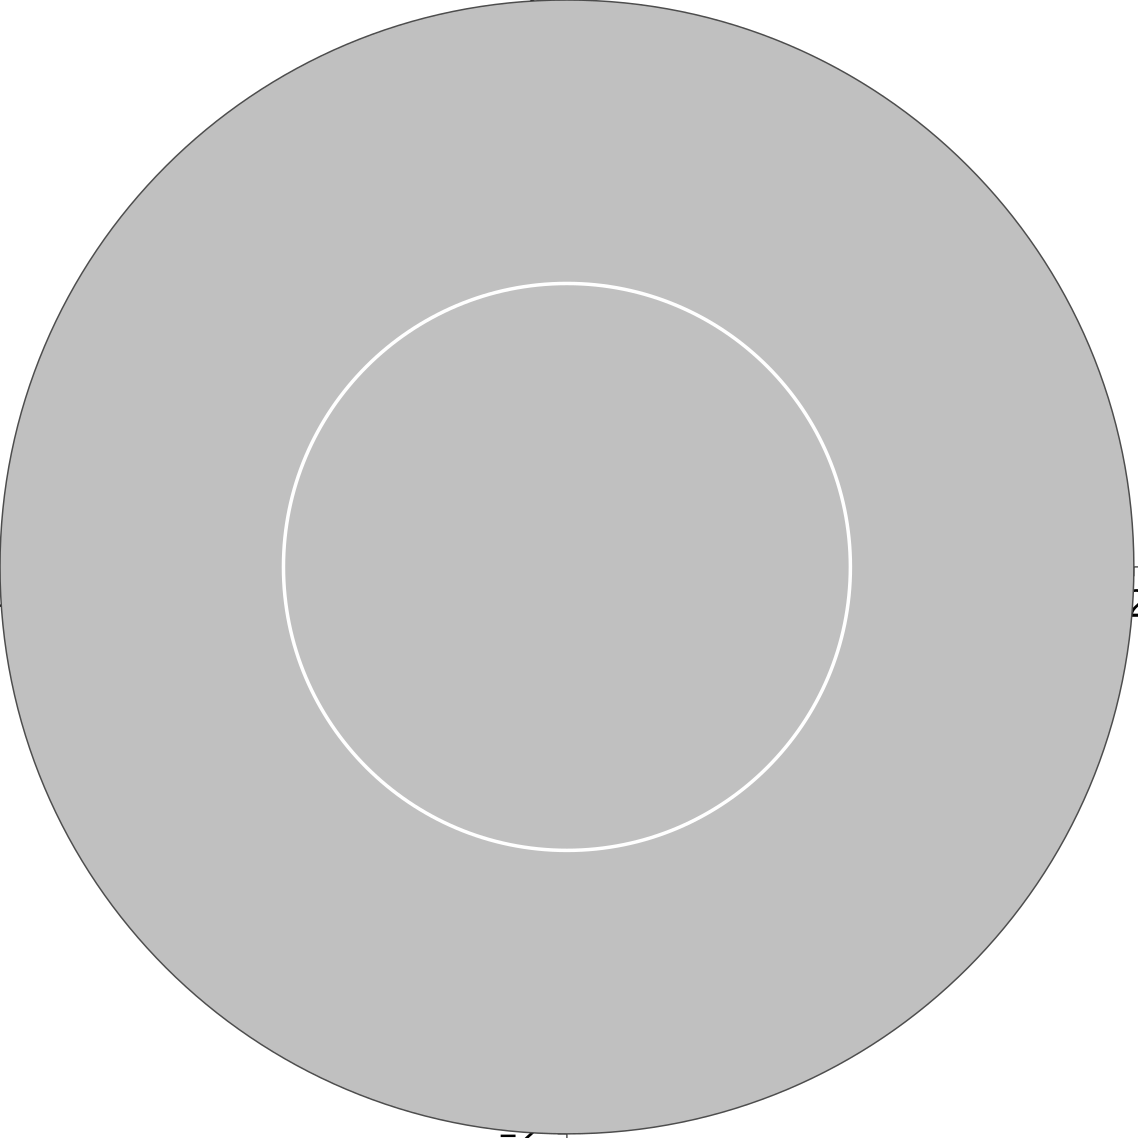
\includegraphics{Cut_set_disk.eps}}
\caption{The disk $D$ and cut set $S$.} 
\label{F:Cut_set_disk}
\end{center}
\end{figure}

\end{enumerate}
\end{example}

Once we have a new property, we then ask if that property is a topological invariant.

\begin{theorem} Let $X$ and $Y$ be connected topological spaces and let $f:X \to Y$ be a homeomorphism. If $S \subset X$ is a cut set, then $f(S)$ is a cut set of $Y$. 
\end{theorem}

\begin{proof} Let $X$ and $Y$ be topological spaces with $f : X \to Y$ a homeomorphism. Let $S$ be a cut set of $X$. Let $U$ and $V$ form a separation of $X \setminus S$. We will demonstrate that $f(U)$ and $f(V)$ form a separation of $Y \setminus f(S)$, which will prove that $f(S)$ is a cut set of $Y$. Since $f^{-1}$ is continuous, the sets $f(U)$ and $f(V)$ are open sets in $Y$. Next we prove that $(Y \setminus f(S)) \subseteq (f(U) \cup f(V))$. Let $y \in Y \setminus f(S)$. Since $f$ is a surjection, there exists an $x \in X$ with $f(x) = y$. The fact that $y \notin f(S)$ means that $x \notin S$. So $x \in (X \setminus S) \subseteq (U \cup V)$. If $x \in U$, then $f(x) = y \in f(U)$ and if $x \in V$, then $x = f(y) \in f(V)$. So $(Y \setminus f(S)) \subseteq (f(U) \cup f(V))$. 

Now we demonstrate that $f(U) \cap (Y \setminus f(S)) \neq \emptyset$ and $f(V) \cap (Y \setminus f(S)) \neq \emptyset$. Since $U$ and $V$ form a separation of $X \setminus S$, we know that $U \cap (X \setminus S) \neq \emptyset$ and $V \cap (X \setminus S) \neq \emptyset$. Let $x \in U \cap (X \setminus S)$. Then $x \in U$ and $x \notin S$. So $f(x) \in f(U)$ and the fact that $f$ is an injection implies that $f(x) \notin f(S)$. Thus, $f(x) \in f(U) \cap (Y \setminus f(S))$. The same argument shows that $x \in V \cap (X \setminus S)$ implies that $f(x) \in f(V) \cap (Y \setminus f(S))$. So $f(U) \cap (Y \setminus f(S)) \neq \emptyset$ and $f(V) \cap (Y \setminus f(S)) \neq \emptyset$. 

Finally, we show that $f(U) \cap f(V) \cap (Y \setminus f(S)) = \emptyset$. Suppose $y \in f(U) \cap f(V) \cap (Y \setminus f(S))$. Let $x \in X$ such that $f(x) = y$. Since $f$ is an injection, we know that $f(x) \in f(U)$ means $x \in U$. so $x \in U \cap V$. The fact that $y \in Y \setminus f(S)$ means that $y \notin f(S)$. Thus, $x \notin S$. So $x \in X \setminus S$. We then have $x \in U \cap V \cap (X \setminus S) = \emptyset$. It follows that $f(U) \cap f(V) \cap (Y \setminus f(S)) = \emptyset$. Therefore, $f(U)$ and $f(V)$ form a separation of $Y \setminus f(S)$ and $f(S)$ is a cut set of $Y$. 

\end{proof}


\begin{activity} ~
\ba
	\item Use the idea of cut sets/points to explain why the unit circle in $\R^2$ is not homeomorphic to the interval $[0,1]$ in $\R$. Note: the unit circle is the set $\{(x,y) \mid x^2+y^2 = 1\}$. Draw pictures to illustrate your explanation. (A formal proof is not necessary, but you need to provide a convincing justification.)

	\item Consider the following subsets of $\R^2$ in the subspace topology: 
\[A = \{ (x,y) \mid x^2+y^2 =1\} \ \ \ \text{ and } \ \ \ B = \{ (x,0) \mid -1 \leq x \leq 1\}.\]
Is $A \cup B$ homeomorphic to $A$? (A formal proof is not necessary, but you need to provide a convincing justification.)
 
\ea

\end{activity}

\begin{comment}

\ActivitySolution

\ba

	\item  Every interior point of the interval $[0,1]$ is a cut point, but the unit circle has no cut points. 

	\item  The answer is no. Any set of two distinct points is a cut set of $A$, but $A \cup B$ has only one set of two points that is a cut set.  
 
\ea

\end{comment}

We have seen that topological equivalence is an equivalence relation, which partitions the collection of all topological spaces into disjoint homeomorphism classes. Topological invariants can then help us identify the classes to which different spaces belong. In general, though, it can be more difficult to prove that two spaces are homeomorphic than not homeomorphic. 

\begin{activity} Consider the spaces $S_1 = \R$, $S_2 = (0,1)$ in $\R$, $S_3 = [-1,1]$ in $\R$, the line segment $S_4$ in $\R^2$ between the points $(0,0)$ and $(2,2)$, the space $S_5$ determined by the letter {\fontfamily{cmss}\selectfont{X}}, and the space $S_6$ determined by the letter {\fontfamily{cmss}\selectfont{Y}} in $\R^2$. Identify the distinct homeomorphism classes determined by these six spaces. No formal proofs are necessary, but you need to give convincing arguments. 

\end{activity}

\begin{comment}

\ActivitySolution We have already shown that $\R$ and $(0,1)$ are homeomorphic spaces. Thus, $[\R] =[(0,1)]$. Since $S_3$ and $S_4$ contain points that are not cut points, we conclude that neither space is in $[\R]$. Removing the center point in $S_5$ cuts $S_5$ into four connected components, and no point in $\R$ does the same. So $S_5 \notin [\R]$. Similarly, removing the middle point from $S_6$ cuts $S_6$ into three connected components. So $S_6 \notin [\R]$. Therefore, only $S_1$ and $S_2$ belong to $[\R]$. 

The function $f: S_3 \to S_4$ defined by $f(x) = (x+1, x+1)$ is linear in both components, so is a homeomorphism. Thus, $[S_3]= [S_4]$. For the same reason as above, neither $S_5$ nor $S_6$ is in $[S_3]$. Therefore, only $S_3$ and $S_4$ are in $[S_3]$. 

Finally, there is no point in $S_5$ that cuts $S_5$ into three connected components, so $[S_5] \neq [S_6]$. We conclude that the distinct classes are $[S_1]$, $[S_3]$, $[S_5]$, and $[S_6]$. 

\end{comment}

\csection{The Intermediate Value Theorem and a Fixed Point Theorem}

In this section we present two important consequences of connectedness. The first consequence is the Intermediate Value Theorem. In calculus, the Intermediate Value Theorem tells us that if $f$ is a continuous function on a closed interval $[a,b]$, then $f$ assumes all values between $f(a)$ and $f(b)$. This result seems straightforward if one just draws a graph of a continuous function on a closed interval. But a picture is not a proof. We state and then prove a more general version of the Intermediate Value Theorem. 

\begin{theorem}[The Intermediate Value Theorem] Let $X$ be a topological space and $A$ a connected subset of $X$. If $f : A \to \R$ is a continuous function, then for any $a,b \in A$ and any $y \in \R$ between $f(a)$ and $f(b)$, there is a point $x \in A$ such that $f(x) = y$. 
\end{theorem}

\begin{activity} In this activity we prove the Intermediate Value Theorem. Let $X$ be a topological space and $A$ a connected subset of $X$. Assume that $f : A \to \R$ is a continuous function, and let $a,b \in A$. \ba
\item Explain why we can assume that $a \neq b$.
  
\item Explain what happens if $y = f(a)$ or $y=f(b)$.

\item Now assume that $f(a) \neq f(b)$. Without loss of generality, assume that $f(a) < f(b)$. Why can we say that $f(A)$ is an interval? 

\item How does the fact that $f(A)$ is an interval complete the proof?

\ea

\end{activity}

\begin{comment}

\ActivitySolution

\ba
\item If $a=b$, then the only $y$ between $f(a)$ and $f(b)$ is $f(a)$, which is a value attained by $f$ on $[a,b]$.
  
\item If $y = f(a)$, then we take $c = a$. If $y = f(b)$, then we take $c=b$. 

\item Since $A$ is connected in $X$, Theorem \ref{thm:connected_invariant} shows that $f(A)$ is a connected subset of $\R$. We proved that the connected subsets of $\R$ are single point sets or intervals. Since $f(a) < f(b)$, we know that $f(A)$ is not a single point set, so $f(A)$ is an interval. 

\item Since $f(A)$ is an interval, it contains all values between $f(a)$ and $f(b)$. So if $f(a) < y < f(b)$, then $y \in f(A)$. 

\ea

\end{comment}


Our second consequence of connectedness involves a fixed point theorem. Fixed point theorems are important in mathematics. A fixed point of a function $f$ is an input $c$ so that $f(c) = c$. There are many fixed point theorems -- one of the most well-known is the Brouwer Fixed Point Theorem that shows that every continuous function from a closed ball $B$ in $\R^n$ to itself must have a fixed point. We can use the Intermediate Value Theorem to prove this result in $\R$. 

\begin{activity} In this activity we prove the following theorem.

\begin{theorem} Let $a,b \in \R$ with $a < b$, and let $f : [a,b] \to [a,b]$ be a continuous function. Then there is a number $c \in [a,b]$ such that $f(c) = c$. 
\end{theorem}

So let $a,b \in \R$ with $a < b$, and let $f : [a,b] \to [a,b]$ be a continuous function.
\ba
\item Explain why we can assume that $a < f(a)$ and $f(b) < b$. 

\item  Define $g : [a,b] \to \R$ by $g(x) = x-f(x)$.
	\begin{enumerate}[i.]
	\item Why is $g$ a continuous function?
	
	\item What can we say about $g(a)$ and $g(b)$? Use the Intermediate Value Theorem to complete the proof.
	
	\end{enumerate}

\item Let $f(x) = \frac{1}{6}x^3+\frac{1}{4}x$.
	\begin{enumerate}[i.]
	\item Show that $f$ maps the interval $[-1,2]$ into the interval $[-1,2]$. (Hint: Use Theorem \ref{thm:max_min} on page \pageref{thm:max_min} that a continuous function from a compact topological space to $\R$ assumes a maximum and minimum value.)
	
	\item Find all values of $c$ in $[-1,2]$ such that $f(c) = c$. 
	
	\end{enumerate}
	
\ea

\end{activity}

\begin{comment}

\ActivitySolution

\ba
\item If $f(a) = a$ or $f(b) = b$, then $f$ has a fixed point and we are done. So we can assume that $f(a) \neq a$ and $f(b) \neq b$. Since $f(a)$ and $f(b)$ are in $[a,b]$, it follows that $a < f(a)$ and $f(b) < b$. 

\item  Define $g : [a,b] \to \R$ by $g(x) = x-f(x)$.
	\begin{enumerate}[i.]
	\item The fact that $g$ is a difference of two continuous functions implies that $g$ is a continuous function. 
	
	\item Now $f(a) > a$ implies $g(a) = a - f(a) < 0$ and $f(b)< b$ implies that $g(b) = b - f(b) > 0$. The Intermediate Value Theorem then tells us that there is a number $c \in [a,b]$ such that $g(c) = 0$. But then 
\[0 = g(c) = c - f(c)\]
and $f(c) = c$. Thus we demonstrated that $f$ must have a fixed point.	

	\end{enumerate}

\item Let $f(x) = \frac{1}{6}x^3+\frac{1}{4}x$.
	\begin{enumerate}[i.]
	\item From calculus, the maximum and minimum values of $f$ occur at an endpoint or at a critical point. The derivative of $f$ is $f'(x) = \frac{1}{2}x^2 + \frac{1}{4}$. Since $f'(x) > 0$ for every $x$, the function $f$ is increasing. That means that the minimum value of $f$ on $[-1,2]$ is $f(-1) = -\frac{5}{12} > -1$ and the maximum value of $f$ on $[-1,2]$ is $f(2) = \frac{11}{6} < 2$.so $f$ maps the interval $[-1,2]$ into the interval $[-1,2]$. 
		
	\item To find such a value for $c$, we solve the equation $f(c) = c$:
	\begin{align*}
	\frac{1}{6}c^3+\frac{1}{4}c &= c \\
	\frac{1}{6}c^3-\frac{3}{4}c &= 0 \\ 
	\frac{1}{2}c\left(\frac{1}{3}c^2-\frac{3}{2}\right).
	\end{align*}
	 
	 So $c = 0$ or $c^2 = \frac{9}{2}$. In the interval $[-1,2]$ we then have $c = 0$ or $c = \frac{3}{\sqrt{2}}$. 
	
	\end{enumerate}
	
\ea


\end{comment}


\csection{Summary}
Important ideas that we discussed in this section include the following.
\begin{itemize}
\item A topological space $(X,\tau)$ is \textbf{connected}\index{connected space} if $X$ cannot be written as the union of two disjoint, nonempty, open subsets. A subset $A$ of a topological space topological space $(X,\tau)$ is connected if $A$ is connected in the subspace topology. 
\item A separation of a subset $A$ of a topological space $X$ is a pair of nonempty open subsets $U$ and $V$ of $X$ such that 
\begin{itemize}
\item $A \subseteq (U \cup V)$,
\item $U \cap A \neq \emptyset$, 
\item $V \cap A \neq \emptyset$, and
\item $U \cap V \cap A = \emptyset$.
\end{itemize}
Showing that a set has a separation can be a convenient way to show that the set is disconnected.
\item The connected subsets of $\R$ are the intervals and the single point sets.
\item A subspace $C$ of a topological space $X$ is a connected component of $X$ if $C$ is connected and there is no larger connected subspace of $X$ that contains $C$.
\item One application of connectedness is the Intermediate Value Theorem that tells us that if $A$ is a connected subset of a topological space $X$ and if $f : A \to \R$ is a continuous function, then for any $a,b \in A$ and any $y \in \R$ between $f(a)$ and $f(b)$, there is a point $x \in A$ such that $f(x) = y$. 
\item A subset $S$ of a connected topological space $X$ is a cut set of $X$ if the set $X \setminus S$ is disconnected, while a .point $p$ in $X$ is a cut point if $X \setminus \{p\}$ is disconnected. The property of being a cut set or a cut point is a topological invariant, so we can sometimes use cut sets and cut points to show that topological spaces are not homeomorphic.
\end{itemize}

\csection{Exercises}

\be

\item Recall from Definition \ref{def:weaker_topologies} on page \pageref{def:weaker_topologies} that if $\tau_1$ and $\tau_2$ are two topologies on a set $X$ such that $\tau_1 \subseteq \tau_2$, then $\tau_1$ is said to be a \emph{coarser} (or \emph{weaker}) topology than $\tau_2$, or $\tau_2$ is a \emph{finer} (or \emph{stronger}) topology than $\tau_1$. In this exercise we explore the question of whether compactness is a property that is passed from weaker to stronger topologies or from stronger to weaker. 

Let $\tau_1$ and $\tau_2$ be two topologies on a set $X$. If $\tau_1 \subseteq \tau_2$, what does connectedness under $\tau_1$ or $\tau_2$ imply, if anything, about compactness under the other topology? Justify your answers.

\begin{comment}

\ExerciseSolution Let $A$ be a subset of $X$.  If $U$ and $V$ form a separation of $A$ in $(X, \tau_1)$, then $U$ and $V$ also form a separation of $A$ in $(X, \tau_2)$. So if $A$ is disconnected in $(X, \tau_1)$, then $A$ is disconnected in $(X, \tau_2)$. In other words, if $A$ is connected in $(X, \tau_2)$, then $A$ is connected in $(X, \tau_1)$. 

However, if $A$ is connected in $(X, \tau_1)$ it does not follow that $A$ is connected in $(X, \tau_2)$. For example, let $X = \R$ with $\tau_1$ the Euclidean metric topology and $\tau_2$ the discrete topology. We know that $A = (0,2)$ is connected in $(X, \tau_1)$. But $U = (0,1]$ and $V = (1,2)$ form a separation of $A$ in $(X, \tau_2)$ and so $A$ is not connected in $(X, \tau_2)$. 

\end{comment}


\item Let $f: [a,b] \to \R$ be a continuous function from a closed interval into the reals. Let $U = f(u)$ and $V = f(v)$ be such that $U \leq f(x) \leq V$ for all $x \in [a,b]$. Prove that there is a $w$ between $u$ and $v$ such that $f(w)(b-a) = \int_a^b f(t) \, dt$. 

\begin{comment}

\ExerciseSolution The Intermediate Value Theorem shows that for any value $t$ between $U$ and $V$ there is a number $s \in [a,b]$ such that $f(s) = t$. From calculus we know that $f(x) \leq V$ on $[a,b]$ implies that 
\[\int_a^b f(t) \, dt \leq \int_a^b V \, dt  = V(b-a)\]
and $U \leq f(x)$ on $[a,b]$ implies that 
\[\int_a^b f(t) \, dt \geq \int_a^b U \, dt  = U(b-a).\]
So 
\[U(b-a) \leq \int_a^b f(t) \, dt \leq V(b-a)\]
or
\[U \leq \frac{1}{b-a} \int_a^b f(t) \, dt \leq V.\]
Therefore, there exists $w \in [a,b]$ such that 
\[f(w) = \frac{1}{b-a} \int_a^b f(t) \, dt\]
or
\[f(w)(b-a) = \int_a^b f(t) \, dt.\]
You may recognize this result from calculus that the area between the graph of $f$ and the $x$-axis on $[a,b]$ can be realized as the area of a rectangle with height $f(w)$ and base $[a,b]$. The value $f(w)$ is the \emph{average value} of $f$ on $[a,b]$. 

\end{comment}

\item Let $A$ be a connected subset of a topological space $X$. Prove or disprove:
\ba
\item $\Int(A)$ is connected

\item $\overline{A}$ is connected

\item $\Bdry(A)$ is connected


\ea

\begin{comment}

\ExerciseSolution

\ba

\item Let $X = \{a,b,c,d,e,f\}$ with topology $\{\emptyset, \{a,b\}, \{c,d\}, \{a,b,e\}, \{c,d,e\}, \{a,b,c,d\}, X\}$. Let $A = \{a,b,c,d,f\}$. The only open set that contains $A$ is $X$, so $A$ is connected. The open sets $\{a,b\}$ and $\{c,d\}$ are contained in $A$, so $a$, $b$, $c$, and $d$ are interior points of $A$.  However, the only open set containing $f$ is $X$, so $f$ is not an interior point of $A$. Thus, $\Int(A) = \{a,b,c,d\} = \{a,b\} \cup \{c,d\}$ and $\Int(A)$ is disconnected.

\item This statement is true by the theorem that states that if $C$ is a subset of $X$ and $A \subseteq C \subseteq \overline{A}$, then $C$ is connected. 

\item Let $A = [0,1]$ in $\R$ with the Euclidean topology. Then $\Bdry(A) = \{0,1\}$ is disconnected.

\ea

\end{comment}


\item Let $X = \R$ with the finite complement topology. We have shown that every subset of any topological space with the finite complement topology is compact. Now find all of the connected subsets of $X$. Prove your result.

\begin{comment}

\ExerciseSolution We know that all single point sets are connected. We will show that a subset $A$ of $\R$ with the finite complement topology is connected if and only if $A$ is a single point set or an infinite set. 

First we demonstrate that every finite subset of $\R$ with two or more points is disconnected under the finite complement topology. Let $A$ be a finite subset of $\R$ containing at least two points $a$ and $b$. Let $U = \R \setminus \{a\}$ and let $V = \R \setminus (A \setminus \{a\})$. Then $U$ and $V$ are open, $A \subseteq U \cup V$, $U \cap A = (A \setminus \{a\}) \neq \emptyset$, $V \cap A = \{a\} \neq \emptyset$, and $U \cap V \cap A = \emptyset$. Thus there exists a separation $U$ and $V$ of $A$ and $A$ is disconnected. 

Now we prove that every infinite set of $\R$ under the finite complement topology is connected. Let $A$ be an infinite subset of $\R$. Proceed by contradiction and assume that $A$ is disconnected. Thus, there exists a separation $U$ and $V$ of $A$. Since $\R \setminus U$ and $\R \setminus V$ are both finite, $U$ and $V$ each contain all but a finite number of elements of the set $A$.  So $U \cap V$ must contain an infinite number of elements of $A$, which makes $U \cap V \cap A$ nonempty. Thus, $A$ is connected. 

\end{comment}

\item Give examples, with justification, of subsets $A$ and $B$ of a topological space to illustrate each of the following, or explain why no such example exists:
\ba
\item $A$ and $B$ are connected, but $A \cap B$ is disconnected

\item $A$ and $B$ are connected, but $A \setminus B$ is disconnected

\item $A$ and $B$ are disconnected, but $A \cup B$ is connected

\item $A$ and $B$ are connected and $A \cap B \neq \emptyset$, but $A \cup B$ is disconnected.

\item $A$ and $B$ are connected and $\overline{A} \cap \overline{B} \neq \emptyset$, but $A \cup B$ is disconnected.

\ea

\begin{comment}

\ExerciseSolution

\ba
\item Let $X = \R^2$ with the Euclidean topology, let $A$ be the line $y=x$, and let $B$ be the parabola $y = x^2$. Both $A$ and $B$ are images of $\R$ via continuous functions and so are connected. However, $A \cap B = \{(0,0), (1,1)\}$, which can be separated by the open balls $B((0,0),1)$ and $B((1,1),1)$. Thus, $A \cap B$ is disconnected.

\item Let $X = \R$ with the Euclidean topology, let $A = [-1,1]$, and let $B = \{0\}$. Then $A \setminus B = [-1,0) \cup (0,1]$ is disconnected. 

\item Let $X = \R$ with the Euclidean topology, let $A = (-1,0] \cup [1,2) \cup [3,4)$, and let $B = (0,1) \cup [2,3)$. Then $A$ and $B$ are disconnected, but $A \cup B = (-1,4)$ is connected. 

\item This is not possible. Suppose $A$ and $B$ are connected, $A \cap B \neq \emptyset$, and suppose that $A \cup B$ is disconnected. Then there is a separation $U$ and $V$ of $A \cup B$. That is, $U$ and $V$ are open sets in $X$ with $U \cap V \cap (A \cup B) = \emptyset$, $U \cap (A \cup B) \neq \emptyset$, $V \cap (A \cup B) \neq \emptyset$, and $A \cup B \subseteq U \cup V$. Let $x \in A \cap B$. Then $x \in U$ or $x \in V$. Without loss of generality assume that $x \in U$. Then $U_A = U \cap A$ is nonempty. We know that $U_A$ is open in $A$. If $V_A = V \cap A$ is also nonempty, then $A \subseteq (U \cup V)$ and $(U \cap V) \cap A \subseteq (U \cap V) \cap (A \cup B) = \emptyset$. So $U$ and $V$ form a separation of $A$. But this is not possible because $A$ is connected. Thus, $V_A = \emptyset$. From this we must have that $U_A = A$. A similar argument shows that $U_B = U \cap B$ is equal to $B$ and $V_B = V \cap B = \emptyset$. Thus, $V \cap (A \cup B) = \emptyset$. We can only conclude that $A \cup B$ is connected. 

\item Let $X = \R$ with the Euclidean topology, let $A = (0,1)$ and $B = (1,2)$. Then $A$ and $B$ are connected intervals with $\overline{A} \cap \overline{B} = [0,1] \cap [1,2] = \{1\}$. But $A \cup B = (0,1) \cup (1,2)$ is disconnected. 
\ea

\end{comment}

\item Let $f: S^1 \to \R$ be a continuous function. Show that there is a point $x \in S^1$ with $f(x) = f(-x)$. 

\begin{comment}

\ExerciseSolution If $f = 0$, then any $x \in S^1$ will do. Suppose $f \neq 0$. Let $g:S^1 \to \R$ be defined by $g(x) = f(x) - f(-x)$. Since $-x$ is a scalar multiple of a continuous function and $g$ is a sum of continuous functions, $g$ is continuous. Let $a \in S_1$ such that $f(a) \neq 0$. If $f(a) = f(-a)$, we are done. So suppose $f(a) \neq f(-a)$. Without loss of generality, assume that $f(a) < f(-a)$. Then $g(a) = f(a) - f(-a) < 0$ and $g(-a) = f(-a) - f(a) > 0$. Since $S^1$ is connected, the Intermediate Value Theorem shows that there is a $y \in S^1$ with $g(y) = 0$. Thus, $f(y) = f(-y)$. 

\end{comment}

\item Let $a, b \in \R$ with $a < b$. Explain why no two of the sets $(a,b)$, $(a,b]$, and $[a,b]$ homeomorphic. 

\begin{comment}

\ExerciseSolution Notice that every point of $(0,1)$ is a cut point, while the point $b$ is not a cut point of $(a,b]$ or $[a,b]$. So $(a,b)$ is not homeomorphic to either $(a,b]$ or $[a,b]$. The set $(a,b]$ has only one point that is not a cut point while $[a,b]$ has two ($a$ and $b$). So $(a,b]$ is not homeomorphic to $[a,b]$. 

\end{comment}

\item Even though $X = (0,1) \cup (1,2)$ is not a connected space, if $x$ is any element in $X$ then we can surround $x$ with a connected subset of $X$.  This is the idea of local connectedness. 

\begin{definition} A topological space $X$ is \textbf{locally connected at a point} $x \in X$ if every neighborhood $U$ of $x$ contains an open connected neighborhood of $x$. A topological space $X$ is \textbf{locally connected}\index{locally connected} if $X$ is locally connected at each point in $X$. 
\end{definition}

\ba

\item Give an example of a locally connected space that is not connected. 

\item It would be reasonable to believe that a connected space is locally connected. However, that is not the case. Consider the space $X = A \cup B$ as a subspace of $\R^2$ with the standard Euclidean metric topology, where $A = \{(x,y) \mid x \text{ is irrational and } 0 \leq y \leq 1\}$ and $B = \{(x,y) \mid x \text{ is rational and } -1 \leq y \leq 0\}$.  
	\begin{enumerate}[i.]
	\item Explain why $X$ is connected.
	
	\item Show that $X$ is not locally connected. (Hint: Let $x$ be a point not on the $x$-axis and find an open ball around $x$ that doesn't intersect the $x$-axis.)
	
	\end{enumerate}
	

\item Prove that a topological space $X$ is locally connected if and only if for every open set $O$ in $X$, the connected components of $O$ are open in $X$.  

\ea

\begin{comment}

\ExerciseSolution

\ba

\item The subspace $X = (0,1) \cup (1,2)$ of $(\R, d_E)$ is not connected, but if $x \in X$ and $O$ is an open set containing $x$, then there is a connected open interval $B(x, r)$  that is contained in $O$. So $X$ is locally connected. 

\item 
	\begin{enumerate}[i.]
	\item The space $X$ consists of vertical line segments with irrational $x$ coordinates when $0 \leq y \leq 1$ and rational $x$ coordinates when $-1 \leq y \leq 0$. These line segments are all connected subsets. Each of these line segments is connected to the entire $x$-axis, which we will label as $L$. So the connected components of $X$ are the sets $\{(x,y) \mid x \text{ is irrational and } 0 \leq y \leq 1\} \cup L$ and $\{(x,y) \mid x \text{ is rational and } -1 \leq y \leq 0\} \cup L$. These sets all contain the line $L$ and the union of these components is $X$. Thus, $X$ is connected. 
	
	\item Consider the point $x = \left(0,\frac{1}{2}\right)$, and let $O = B\left(x,\frac{1}{4}\right)$. Then $O \cap L = \emptyset$. So $O$ is a union of vertical line segments that do not connect with the $x$-axis. Let $U$ be a neighborhood of $x$ in $O$. Then there is real number $r > 0$ such that $B(x,r) \subseteq U$. But $B(x,r)$ contains points $(a,0)$ and $(-a,0)$ with $a$ irrational. But the connected components of these two points form a disconnected set. So $U$ cannot be connected. We conclude that $X$ is not locally connected. 
	
	\end{enumerate}
	
\item Let $X$ be a locally connected topological space and let $O$ be an open set in $X$. Let $C$ be a connected component of $O$. Since $X$ is locally connected and $O$ is a neighborhood of $x$, there is a connected open neighborhood $U$ of $x$ contained in $O$. Since $C$ is a connected component, it follows that $U \subseteq C$. So $C$ contains a neighborhood of $x$ and is therefore a neighborhood of each of its points. We conclude that $C$ is open.

Conversely, assume that for each open set $O$, the connected components of $O$ are open in $X$. To show that $X$ is locally  connected, let $x \in X$ and let $N$ be a neighborhood of $x$. Let $O$ be an open set in $N$ that contains $x$ and let $C$ be the connected component of $O$ containing $x$. By hypothesis, $C$ is open in $X$. Thus, $C$ is a connected open neighborhood of $x$ in $X$. So $X$ is locally connected at each point and is therefore locally connected. 


\ea



\end{comment}

\item Let $A$ and $B$ be nonempty subsets of a topological space $X$. 
\ba
\item Prove that $A \cup B$ is disconnected if $(\overline{A} \cap B ) \cup (A \cap \overline{B}) = \emptyset$. 
\item Prove that $X$ is connected if and only if for every pair of nonempty subsets $A$ and $B$ of $X$ such that $X = A \cup B$ we have $(\overline{A} \cap B ) \cup (A \cap \overline{B}) \neq \emptyset$.

\ea

\begin{comment}

\ExerciseSolution 
\ba
\item Let $A$ and $B$ be nonempty subsets of a space $X$. Assume that $(\overline{A} \cap B ) \cup (A \cap \overline{B}) = \emptyset$. Then  $\overline{A} \cap B  = \emptyset$ and $A \cap \overline{B} = \emptyset$. Note that 
\[(A \cap B) \subseteq (\overline{A} \cap B) = \emptyset,\]
so $A$ and $B$ must be disjoint. Let $U = X \setminus \overline{A}$ and $V = X \setminus \overline{B}$. We will show that $U$ and $V$ form a separation of $A$ and $B$. Since closures are closed sets, we know that $U$ and $V$ are open sets. We know that $B$ is nonempty, and $\overline{A} \cap B = \emptyset$, so $B \subseteq U$. Similarly, $A \subseteq V$. So $(A \cup B) \subseteq (U \cup V)$. To complete the proof, we see that $A \subseteq \overline{A}$, so $A \cap U = \emptyset$. Similarly, $B \cap V = \emptyset$. So
\[U \cap V \cap (A \cup B) = (U \cap V \cap A) \cup (U \cap V \cap B) = \emptyset.\]
Therefore, $A$ and $B$ are disconnected. 

\item Assume that $X$ is a connected topological space, and let $A$ and $B$ be nonempty subsets of $X$ with $A \cup B = X$. By the first part of the problem, if $(\overline{A} \cap B ) \cup (A \cap \overline{B}) = \emptyset$, then $A \cup B = X$ is disconnected. We conclude that $(\overline{A} \cap B ) \cup (A \cap \overline{B}) \neq \emptyset$.

Finally, assume that for any nonempty subsets $A$ and $B$ of $X$ such that $X = A \cup B$ we have $(\overline{A} \cap B ) \cup (A \cap \overline{B}) \neq \emptyset$. To prove that $X$ is connected, we will show that $X$ contains no non-trivial subset that is both open and closed. We proceed by contradiction and assume that there is a nonempty proper subset $A$ of $X$ that is both open and closed. Then $X \setminus A$ is also open and closed. Since $A$ and $X \setminus A$ are not empty and $X = A \cup (X \setminus A)$, our hypothesis tells us that $(\overline{A} \cap (X \setminus A) ) \cup (A \cap \overline{X \setminus A}) \neq \emptyset$.  But $A$ and $X \setminus A$ are closed, so we have $(A \cap (X \setminus A)) \neq \emptyset$, which cannot happen. We conclude that $X$ contains no non-trivial subset that is both open and closed, or that $X$ is connected. 

\ea

\end{comment}

\item Give examples of the following.
\ba
\item A topological space with exactly one cut point.

\item A topological space with exactly two cut points.

\item A topological space with infinitely many cut points.
 
\item A topological space with no cut points.

\ea

\begin{comment}

\ExerciseSolution

\ba
\item Consider $X$ as a subset of $\R^2$ to be the set consisting of two loops that are tangent at point $a$. No point on either loop, except $a$ is a cut point. However, $X \setminus \{a\}$ is a disconnected union of two circles minus a point. 

\item Consider $X$ as a collection of three loops $L_1$, $L_2$, and $L_3$ such that $L_1$ and $L_2$ are tangent at point $a$, $L_2$ and $L_3$ are tangent at point $b$, and $L_1$ and $L_3$ do not intersect. As in part (a), the only cut points are the points of tangency.

\item Consider a line segment. Every point, except the endpoints, is a cut point. 
 
\item A circle has no cut points. 

\ea

\end{comment}


\item Let $a, b \in \R$ with $a < b$. Prove that a homeomorphism $f: [a,b] \to [a,b]$ carries end points into end points. 

\begin{comment}

\ExerciseSolution Let $a,b \in \R$ with $a < b$. Let $A = [a,b]$, and let $f: A to A$ be a homeomorphism. Notice that if $a < c < b$ for some real number $c$, then $A \setminus \{c\} = [a,c) \cup (c,b]$ and $A \setminus \{c\}$ is disconnected. Thus, every $c$ strictly between $a$ and $b$ is a cut point of $A$. Note also that $A \setminus \{a\} = (a,b]$ and $A \setminus \{b\} = [a,b)$, and $A \setminus \{a\}$ and $A \setminus \{b\}$ are intervals. So  $A \setminus \{a\}$ and $A \setminus \{b\}$ are connected. Thus, $a$ and $b$ are not cut points of $A$. Since a homeomorphism must preserve cut points, it follows that $f(a)$ must be either $a$ or $b$ and $f(b)$ must be either $a$ or $b$. Thus, $f$ sends endpoints to endpoints. 


\end{comment}


\item Let $X$ and $Y$ be a topological spaces.
\ba
\item Assume that $X$ and $Y$ homeomorphic spaces. Prove that there is a one-to-one correspondence between the connected components of $X$ and the connected components of $Y$. 

\item Assume that $X$ and $Y$ homeomorphic spaces. Prove that there is a one-to-one correspondence between the set of cut points of $X$ and the set of cut points of $Y$. 

\item Consider each letter in the statement as a topological space with the standard Euclidean metric topology.
\begin{center} {\fontfamily{cmss}\selectfont TOPOLOGY IS NEAT} \end{center}
Group the letters in the statement into disjoint homeomorphism classes. Explain in detail the reasons for your groupings. 
\ea

\begin{comment}

\ExerciseSolution

\ba

\item Let $f: X \to Y$ be a homeomorphism. Let $C(X)$ be the set of connected components of $X$ and $C(Y)$ the set of connected components of $Y$. Since $f$ is continuous, we know that $f(A)$ is connected in $Y$ whenever $A$ is connected in $X$. Define $g: C(X) \to C(Y)$ by $g(A) = f(A)$. We will show that $g$ is a bijection. 

Suppose $A$ and $B$ are in $C(X)$ and that $g(A) = g(B)$. Then $f(A) = f(B)$. Since $f$ is a bijection we know that $f$ is invertible. Then $f^{-1}(f(A)) = f^{-1}(f(B))$ implies that $A = B$. So $g$ is an injection. 

Now let $D \in C(Y)$. The fact that $f^{-1}$ is continuous shows that $f^{-1}(D)$ is connected in $X$. Thus, $f^{-1}(D) \in C(X)$ and $f(f^{-1}(D)) = D$. So $g$ is a surjection.

\item Let $f: X \to Y$ be a homeomorphism. Let $C(X)$ be the set of cut points of $X$ and $C(Y)$ the set of cut points of $Y$. Since $f$ is continuous, we know that $f(c)$ is a cut point in $Y$ whenever $c$ is a cut point in $X$. Define $g: C(X) \to C(Y)$ by $g(c) = f(c)$. We will show that $g$ is a bijection. 

Suppose $a$ and $b$ are in $C(X)$ and that $g(a) = g(b)$. Then $f(a) = f(b)$. Since $f$ is an injection, it follows that $a = b$. So $g$ is an injection. 

Now let $d \in C(Y)$. The fact that $f^{-1}$ is continuous shows that $f^{-1}(d)$ is a cut point in $X$. Thus, $f^{-1}(d) \in C(X)$ and $f(f^{-1}(d)) = d$. So $g$ is a surjection.

 \begin{itemize}
\item The letter O is the only letter in our list with no cut points. So O forms its own class.

\item The letters P and A are the only letters that have points that are not end points and not cut points. However, if we remove the point joining the leg of P to its head, as shown here \raisebox{-0.085cm}{\includegraphics[height=12pt]{Letter_P.eps}}, one of the resulting connected components (the head) has no cut points. There is no way we can remove only one point from A and have a component with no cut points. So P and A form two separate classes. 
	

\item From part (a), any two homeomorphic spaces will have the same number of connected components. Now each cut point cuts  L, G, I, S, and N into 2 connected components. But in T, Y, or E we can find cut points that cut the sets into more than 2 connected components. So these two groups form at least two different homeomorphism classes. 

	\begin{itemize}
	\item Any one of L, G, S, or N can be continuously deformed into I by pulling on the endpoints. So these letters all fit into the same class.

	\item We can get any one of T, Y, or E from any other by bending, stretching and contracting, so these letters all fit into the same class. For example, to get from E to T  we unfold the top and bottom arms of the letter E. This makes a T that is stretched horizontally and compressed vertically. By stretching and compressing we can get to the letter T.
	\end{itemize}

\end{itemize}

So the the distinct homeomorphism classes are  $\{O\}$, $\{P\}$, $\{A\}$, $\{L, G, I, S, N\}$, and $\{T, Y, E\}$.  

%\ea

\end{comment}

\item Let $(X, \tau)$ be a topological space.
\ba
\item Prove that $X$ is disconnected if and only if $X$ has a proper subset that is both open and closed.
\item Prove that $X$ is disconnected if and only if there is a continuous function from $X$ onto a discrete two-point topological space. 
\ea

\begin{comment}

\ExerciseSolution

\ba

\item  First suppose that $X$ is disconnected. Then there are nonempty disjoint open sets $A$ and $B$ such that $X = A \cup B$. This implies that $X \setminus A = B$ and so $A$ is also closed. Thus, $A$ is both open and closed. 

Now suppose that $A$ is a proper subset of $X$ that is both open and closed. Then $B = X \setminus A$ is open and $X$ is the disjoint union of $A$ and $B$. Thus, $X$ is disconnected. 

\item First suppose that $X$ is disconnected. Then there are nonempty disjoint open sets $A$ and $B$ such that $X = A \cup B$. Let $Y = \{a,b\}$ with the discrete topology. Define $f: X \to Y$ by 
\[f(x) = \begin{cases} a &\text{ if } x \in A \\ b & \text{ if } x \in B.\end{cases}\]
 By definition, $f$ is a surjection. Note that $f^{-1}(\{a\}) = A$ and $f^{-1}(\{b\}) = B$, so $f^{-1}$ of any open set in $Y$ is open in $X$ and $f$ is continuous. 

Now suppose that there is a continuous surjection $f$ from $X$ to a two-point topological space $Y = \{a,b\}$ with the discrete topology. Let $A = f^{-1}(\{a\})$ and $B = f^{-1}(\{b\}$. Since $f$ is continuous, we know that $A$ and $B$ are open in $X$. The fact that $f$ is a surjection means that $A$ and $B$ are nonempty. Since every $x \in X$ maps to either $a$ or $b$, we conclude that $X = A \cup B$. Finally, we show that $A \cap B = \emptyset$. Suppose $x \in A \cap B$. Then $f(x) \in A$ and $f(x) \in B$. This implies that $f(x) = a$ and $f(x) = b$, and $a=b$.  This is impossible because $f$ is a function. Therefore, $X$ is disconnected. 

\ea

\end{comment}


\item Let $X$ be the set of real numbers. 
\ba
\item Consider $X$ with the topology $\tau_1 = \{\emptyset, [0,1], X\}$. Prove or disprove: $X$ is connected.

\item Consider $X$ with the topology $\tau_2 = \{U \subseteq X \mid 0 \in U\} \cup \{\emptyset\}$. 
	\begin{enumerate}[i.]
	\item Prove or disprove: $X$ is connected.
	
	\item Prove or disprove: $X \setminus \{0\}$ is connected.
	
	\end{enumerate}

\ea

\begin{comment}

\ExerciseSolution

\ba

\item The only open set that contains $X$ is $X$ itself, so there is no separation of $X$. Thus, $X$ is connected.

\item Consider $X$ with the topology $\tau_2 = \{U \subseteq X \mid 0 \in U\} \cup \{\emptyset\}$. 
	\begin{enumerate}[i.]
	\item If $U$ and $V$ are open sets, then $0 \in U$ and $0 \in V$. So $0 \in U \cap Y \cap X$. Thus, there is no separation of $X$ and $X$ is connected. 
	
	\item Let $Y = X \setminus \{0\}$, and let $U = \R^+ \cup \{0\}$ and $V = \R^- \cup \{0\}$. Then $U \cap Y \neq \emptyset$, $V \cap Y \neq \emptyset$, $Y \subseteq U \cup V$, and $U \cap V \cap Y = \emptyset$. So $U$ and $V$ form a separation of $Y$ and $Y$ is disconnected. 
	
	\end{enumerate}

\ea

\end{comment}

\item \label{ex:particular_point_connected} Let $X$ be a nonempty set and let $p$ be a fixed element in $X$. Let $\tau_p$ be the particular point topology and $\tau_{\overline{p}}$ the excluded point topology on $X$. That is
\begin{itemize}
\item $\tau_{p}$ is the collection of subsets of $X$ consisting of $\emptyset$, $X$, and all of the subsets of $X$ that contain $p$.  
\item $\tau_{\overline{p}}$ is the collection of subsets of $X$ consisting of $\emptyset$, $X$, and all of the subsets of $X$ that do not contain $p$.
\end{itemize}
That the particular point and excluded point topologies are topologies is the subject of Exercises (\ref{ex:particular_point_topology}) and (\ref{ex:excluded_point_topology}) on page \pageref{ex:particular_point_topology}. 

Determine, with proof, the connected subsets of $X$ when 
\ba
\item $X$ has the particular point topology $\tau_p$

\item $X$ has the excluded point topology $\tau_{\overline{p}}$. 

\ea

\begin{comment}

\ExerciseSolution

	\ba
	\item Let $C$ be a nonempty subset of $X$. We show that $C$ is connected if and only if $p \in C$. Suppose $p \notin C$. Suppose $C_0$ is a subset of $C$. Then $C_0 \cup \{p\}$ is an open set in $X$ and $C \cap (C_0 \cup \{p\}) = C_0$. So the subspace topology on $C$ is the discrete topology. It follows that $C$ is disconnected. 
	
Now suppose that $p \in C$. To show that $C$ is connected, assume that $U$ and $V$ are open sets with $C \subset (U \cup V)$. Since $U$ and $V$ are open, they both contain $p$. From this it follows that $p \in U \cap V \cap C$. So $U$ and $V$ cannot form a separation of $C$ and $C$ is connected.  
		
	\item Let $C$ be a nonempty subset of $X$. We show that $C$ is connected if and only if $p \in C$. Suppose $p \notin C$. Then every subset of $C$ is an open set and the subspace topology on $C$ is the discrete topology. It follows that $C$ is disconnected.
	
Now suppose that $p \in C$. If $U$ and $V$ are open sets in $X$ with $C \subseteq (U \cup V)$, then $p \in (U \cup V)$. But this implies that $p \in U$ or $p \in V$, which is impossible. So $U$ and $V$ cannot form a separation of $C$ and $C$ is connected.  

	
	\ea	

\end{comment}

\item Let $(X, \tau)$ be a topological space and $A$ a connected subset of $X$.

\ba

\item Show that if $X$ is Hausdorff, then $A'$ is connected.

\item Let $(X, \tau) = (\R, \tau_0)$, where $\tau_0$ is the particular point topology on $X$. Explain why $A = \Z$ is a connected subset of $X$. Find $\Z'$ in $(\R, \tau_0)$. Is it true that in any topological space, if $A$ is connected, then so is $A'$? Explain. (See Exercise \ref{ex:particular_point_connected}.) 

\ea


\begin{comment}

\ExerciseSolution

\ba

\item If $A$ is a single point set, then $A' = \emptyset$, which is connected. So assume that $A$ contains more than just one point. First we demonstrate that every point of $A$ is a limit point of $A$. Let $a \in A$. Proceed by contradiction and assume that $a$ is not a limit point of $A$. Then there is an open set $U$ containing $a$ with $U \cap A = \{a\}$. Let $V = X \setminus \{a\}$. Since $X$ is Hausdorff, $\{a\}$ is closed. So $V$ is open. Also, $V \cap A \neq \emptyset$, $U \cap A \neq \emptyset$, and $U \cap V \cap A = \emptyset$. So $U$ and $V$ form a separation of $A$. But this is impossible if $A$ is connected. We conclude that every point of $A$ is a limit point of $A$. Then $\overline{A} = A \cup A' = A'$, which is connected.


\item Exercise \ref{ex:particular_point_connected} shows that the nonempty connected subsets of $(\R, \tau_0)$ are the subsets that contain $0$. So $\Z$ is connected. Now we determine $\Z'$. Let $x \in \R$ with $x \neq 0$. Every open set in $(\R, \tau_0)$ contains $0$, so every open set that contains $x$ also contains a point in $\Z$ that is different from $x$. Thus, every number except $0$ is in $\Z'$. However, the open set $\{0\}$ does not contain any points in $\Z$ different from $0$, so $0 \notin \Z'$. Since $\Z'$ does not contain $0$, we conclude that $\Z'$ is not connected. 

\ea

\end{comment}



\item Let $X$ be a topological space. Prove each of the following.
\ba
\item Each $a \in X$ is an element of exactly one connected component $C_a$ of $X$.
\item A component $C_a$ contains all connected subsets of $X$ that contain $a$. Thus, $C_a$ is the union of all connected subsets of $X$ that contain $a$. 
\item If $a$ and $b$ are in $X$, then either $C_a = C_b$ or $C_a \cap C_b = \emptyset$. 
\item Every connected subset of $X$ is a subset of a connected component.
\item Every connected component of $X$ is a closed subset of $X$.
\item The space $X$ is connected if and only if $X$ has exactly one connected component.
\ea

\begin{comment}

\ExerciseSolution

\ba
\item Let $a \in X$. We know that $\{a\}$ is closed, so there is a largest connected set $C_a$ that contains $a$. Thus, $C_a$ is a connected component. The fact that components are either equal or disjoint implies that $a$ is in exactly one connected component.
\item Since $C_a$ is the largest connected set that contains $a$, every connected set that contains $a$ is a subset of $C_a$. Let $\{K_{\alpha}\}_{\alpha \in I}$ be the collection of connected sets that contain $a$. We know that $K_{\alpha} \subseteq C_a$, so $\bigcup_{\alpha \in I} K_{\alpha} \subseteq C_a$. Now let $x \in C_a$. Let $C_x$ be the connected component of $x$. Since $x \in C_a$, it must be the case that $x \in C_a$. So $C_x = K_{\beta}$ for some $\beta$ and so $C_a \subseteq \bigcup_{\alpha \in I} K_{\alpha}$. Thus, $C_a$ is the union of all connected subsets of $X$ that contain $a$. 
\item Let $a, b \in X$. If $b \in C_a$, then the fact that equivalence classes are either equal or disjoint implies that $C_a = C_b$. If $b \notin C_a$, then the same fact shows that $C_a \cap C_b = \emptyset$. 
\item Let $C$ be a connected subset of $X$. If $C = \emptyset$, then $C$ is itself a connected component. If $a \in C$, then $C$ must be contained in $C_a$ by part (b). 
\item Let $C$ be a connected component of $X$. We know that $\overline{C}$ is also connected. The fact that $C$ is a connected component means that $\overline{C} \subseteq C$. Thus, $C = \overline{C}$ and $C$ is closed.  
\item If $X = \emptyset$, then $X$ is connected and has only one connected component. Suppose $X$ is not empty and connected. Let $x \in X$. Since $X$ is the largest connected set containing $x$, it follows that $C_x = X$. Since connected components are either equal or disjoint, we conclude that $C_x = X$ is the only connected component of $X$. 

Now suppose that $X$ has only one connected component $C$. Then for every $x \in X$ we have that $C_x = C$. Thus, $X \subseteq C$ and so $X = C$ and $X$ is connected. 

\ea

\end{comment}

\item Let $X$ be a topological space with only a finite number of connected components. Show that each component of $X$ is open. 

\begin{comment}

\ExerciseSolution Let $C_1$, $C_2$, $\ldots$, $C_n$ be the distinct components of $X$. We know that each connected component is closed since $\overline{C_i}$ is connected and so $\overline{C_i} \subseteq C_i$. Let $i$ be between $1$ and $n$, and let $K_i = \bigcup_{j \neq i} C_j$. We know that $K_i$ is a closed set. Since $X$ is the disjoint union of the $C_i$, it follows that $C_i = X \setminus K_i$, and so $C_i$ is open. 

\end{comment}


\item Let $X$ and $Y$ be connected spaces with $f : X \to Y$ a continuous function. Is it the case that if $S$ is a cut set of $X$, then $f(S)$ is a cut set of $Y$? Prove your answer.

\begin{comment}

\ExerciseSolution The answer is no. Let $X = [0,1]$ in $\R$ and $Y = \{(x,y) \in \R^2 \mid x^2+y^2 = 1\}$. Define $f: X \to Y$ by $f(t) = (\cos(2 \pi t), \sin(2 \pi t))$. The inverse image of a basic open arc not containing $(1,0)$ in $Y$ is an open interval in $X$, while the inverse image of an open arc that contains $(1,0)$ in $Y$ is a set of the form $[0,s) \cup (t,1]$, which is open in $X$. So $f$ is a continuous function. However, $0.5$ is a cut point of $X$ while $f(0.5)$ is not a cut point of $Y$. 


\end{comment}


\item Let $X = \{a,b,c,d\}$. There are 355 distinct topologies on $X$, but they fit into the 33 distinct homeomorphism classes listed below. The list is ordered by decreasing number of singleton sets in the topology, and, when that is fixed, by increasing number of two-point subsets and then by increasing number of three-point subsets. Under which topologies is $X$ connected? Prove your answer. 

\begin{enumerate}[1.]
\item the discrete topology
\item $\{\emptyset, \{a\}, \{b\}, \{c\}, \{a,b\}, \{a,c\}, \{b,c\}, \{a,b,c\}, X\}$
\item $\{\emptyset, \{a\}, \{b\}, \{c\}, \{a,b\}, \{a,c\}, \{b,c\}, \{a,b,c\}, \{a,b,d\}, X\}$
\item $\{\emptyset, \{a\}, \{b\}, \{c\}, \{a,b\}, \{a,c\}, \{b,c\}, \{a,d\}, \{a,b,c\}, \{a,b,d\}, \{a,c,d\}, X\}$
\item $\{\emptyset, \{a\}, \{b\}, \{a,b\}, X\}$
\item $\{\emptyset, \{a\}, \{b\}, \{a,b\}, \{a,b,c\}, X\}$
\item $\{\emptyset, \{a\}, \{b\}, \{a,b\}, \{a,c,d\}, X\}$
\item $\{\emptyset, \{a\}, \{b\}, \{a,b\}, \{a,b,c\}, \{a,b,d\}, X\}$
\item $\{\emptyset, \{a\}, \{b\}, \{a,b\}, \{a,c\}, \{a,b,c\}, X\}$
\item $\{\emptyset, \{a\}, \{b\}, \{a,b\}, \{a,c\}, \{a,b,c\}, \{a,c,d\}, X\}$
\item $\{\emptyset, \{a\}, \{b\}, \{a,b\}, \{a,c\}, \{a,b,c\}, \{a,b,d\}, X\}$
\item $\{\emptyset, \{a\}, \{b\}, \{a,b\}, \{c,d\}, \{a,c,d\}, \{b,c,d\}, X\}$
\item $\{\emptyset, \{a\}, \{b\}, \{a,b\}, \{a,c\}, \{a,d\}, \{a,b,c\}, \{a,b,d\}, X\}$
\item $\{\emptyset, \{a\}, \{b\}, \{a,b\}, \{a,c\}, \{a,d\}, \{a,b,c\}, \{a,b,d\}, \{a,c,d\}, X\}$
\item $\{\emptyset, \{a\}, X\}$
\item $\{\emptyset, \{a\}, \{a,b\}, X\}$
\item $\{\emptyset, \{a\}, \{a,b\}, \{a,b,c\}, X\}$
\item $\{\emptyset, \{a\}, \{b,c\}, \{a,b,c\}, X\}$
\item $\{\emptyset, \{a\}, \{a,b\}, \{a,c,d\}, X\}$
\item $\{\emptyset, \{a\}, \{a,b\}, \{a,b,c\}, \{a,b,d\}, X\}$
\item $\{\emptyset, \{a\}, \{b,c\}, \{a,b,c\}, \{b,c,d\}, X\}$
\item $\{\emptyset, \{a\}, \{a,b\}, \{a,c\}, \{a,b,c\}, X\}$
\item $\{\emptyset, \{a\}, \{a,b\}, \{a,c\}, \{a,b,c\}, \{a,b,d\}, X\}$
\item $\{\emptyset, \{a\}, \{c,d\}, \{a,b\}, \{a,c,d\}, X\}$
\item $\{\emptyset, \{a\}, \{a,b\}, \{a,c\}, \{a,d\}, \{a,b,c\}, \{a,b,d\}, \{a,c,d\}, X\}$
\item $\{\emptyset, \{a\}, \{a,b,c\}, X\}$
\item $\{\emptyset, \{a\}, \{b,c,d\}, X\}$
\item $\{\emptyset, \{a,b\}, X\}$
\item $\{\emptyset, \{a,b\}, \{c,d\}, X\}$
\item $\{\emptyset, \{a,b\}, \{a,b,c\}, X\}$
\item $\{\emptyset, \{a,b\}, \{a,b,c\}, \{a,b,d\}, X\}$
\item $\{\emptyset, \{a,b,c\}, X\}$
\item $\{\emptyset, X\}$
\end{enumerate}

\begin{comment}

\ExerciseSolution In 2,5,6,9,15,16,17,18,22,26,28,30,32, and 33, the only open set that contains $d$ is $X$, so $X$ cannot be written as a union of disjoint open sets and $X$ is connected under these topologies. We consider the remaining topologies in turn.
\begin{enumerate}
\item[1.] Since $X = \{a,b\} \cup \{c,d\}$, it follows that $X$ is disconnected.

\item[3.] In this case $X = \{c\} \cup \{a,b,d\}$ and so $X$ is disconnected. 

\item[4.] In this case $X = \{b\} \cup \{a,c,d\}$ and so $X$ is disconnected. 

\item[7.]  In this case $X = \{b\} \cup \{a,c,d\}$ and so $X$ is disconnected. 

\item[8.] The only open sets that contains $d$ are $\{a,b,d\}$ and $X$, and each of these sets has a nontrivial intersection with every other open set. So $X$ cannot be written as a union of disjoint open sets and so $X$ is connected. 

\item[10.] In this case $X = \{b\} \cup \{a,c,d\}$ and so $X$ is disconnected.  

\item[11.] The only open sets that contains $d$ are $\{a,b,d\}$ and $X$, and each of these sets has a nontrivial intersection with every other open set. So $X$ cannot be written as a union of disjoint open sets and so $X$ is connected. 

\item[12.] In this case $X = \{b\} \cup \{a,c,d\}$ and so $X$ is disconnected.  

\item[13.] The only pairs of nontrivial disjoint open sets are $\{a\}$ and $\{b\}$, $\{b\}$ and $\{a,c\}$, and $\{b\}$ and $\{a,d\}$. Since no unions of these pairs of disjoint open sets equals $X$, we conclude that $X$ is connected. 

\item[14.] In this case $X = \{b\} \cup \{a,c,d\}$ and $X$ is disconnected. 

\item[19.] Every nonempty open set contains $a$, and so $X$ cannot be written as a disjoint union of open sets. Thus, $X$ is connected. 

\item[20.] Every nonempty open set contains $a$, and so $X$ cannot be written as a disjoint union of open sets. Thus, $X$ is connected. 

\item[21.] In this case $X = \{a\} \cup \{b,c,d\}$ and $X$ is disconnected. 

\item[23.] Every nonempty open set contains $a$, and so $X$ cannot be written as a disjoint union of open sets. Thus, $X$ is connected.  

\item[24.] In this case $X = \{a,b\} \cup \{c,d\}$ and $X$ is disconnected. 

\item[25.] Every nonempty open set contains $a$, and so $X$ cannot be written as a disjoint union of open sets. Thus, $X$ is connected. 

\item[27.] In this case $X = \{a\} \cup \{b,c,d\}$ and $X$ is disconnected. 

\item[29.] In this case $X = \{a,b\} \cup \{c,d\}$ and $X$ is disconnected. 

\item[31.] The only open sets that contains $d$ are $\{a,b,d\}$ and $X$, and each of these sets has a nontrivial intersection with every other open set. So $X$ cannot be written as a union of disjoint open sets and $X$ is connected. 

\end{enumerate}

\end{comment}


\item For each of the following, answer true if the statement is always true. If the statement is only sometimes true or never true, answer false and provide a concrete example to illustrate that the statement is false. If a statement is true, explain why. 
	\ba
	\item If $A$ is a connected subset of a topological space $X$ with $|A| \geq 2$, then every point of $A$ is a limit point of $A$.

\item If $A$ is a compact subspace of a Hausdorff space, then $A$ is connected.

\item If $A$ is a connected subspace of a Hausdorff space, then $A$ is compact.

\item Every subset of a topological space with the discrete topology is disconnected. 

\item The set $\{a,b\}$ is a connected component of the topological space $X = \{a,b,c,d\}$ with topology 
\[\tau = \{\emptyset, \{a\}, \{a,b\}, \{c\}, \{d\}, \{c,d\}, \{a,c,d\}, \{a,c\}, \{a,d\}, \{a,b,c\}, \{a,b,d\}, X\}.\]

\item The sets $U = \{a,c,d\}$ and $V = \{a,b,c\}$ form a separation of the set $A = \{c,d\}$ in the topological space $X = \{a,b,c,d\}$ with topology 
\[\tau = \{\emptyset, \{a\}, \{a,b\}, \{c\}, \{d\}, \{c,d\}, \{a,c,d\}, \{a,c\}, \{a,d\}, \{a,b,c,\}, \{a,b,d\}, X\}.\]

\item The connected topological space $X = \{a,b,c,d\}$ with topology 
\[\tau = \{\emptyset, \{a\}, \{b,c\}, \{a,b,c\}, X\}\]
has no cut points. 
		
	\ea

\begin{comment}

\ExerciseSolution

\ba

\item This statement is true. Let $a \in A$. Proceed by contradiction and assume that $a$ is not a limit point of $A$. Then there is an open set $U$ containing $a$ with $U \cap A = \{a\}$. Let $V = X \setminus \{a\}$. Since $\{a\}$ is closed, $V$ is open. Also, $V \cap A \neq \emptyset$, $U \cap A \neq \emptyset$, and $U \cap V \cap A = \emptyset$. So $U$ and $V$ form a separation of $A$. But this is impossible if $A$ is connected. 

\item This statement is false. Let $X = \R$ with the Euclidean metric topology. Then $X$ is Hausdorff. Let $A = \{0,1\}$. Since $A$ is closed and bounded, $A$ is compact. However, $A$ is not connected because $B(0,1)$ and $B(1,1)$ form a separation of $A$. 

\item This statement is false. Let $X = \R$ with the Euclidean metric topology. Then $X$ is Hausdorff. Let $A = (0,1)$. Then $A$ is connected, but not closed. So $A$ is not compact. 

\item This statement is false, since single point sets are connected. However, every subset having at least two element in a topological space with the discrete topology is disconnected. To see why, let $A$ be a subset of a topological space $X$ such that $|A| \geq 2$. Let $a \in A$. Then $U = \{a\}$ and $V = X \setminus \{a\}$ form a separation of $A$. 	

\item This statement is true. The set $\{a,b\}$ is connected, and $\{a,b,c\} = \{a,b\} \cup \{c\}$, $\{a,b,d\} = \{a,b\} \cup \{d\}$, and $X = \{a,b,c\} \cup \{d\}$ are all disconnected.

\item This statement is false since $U \cap V \cap A = \{c\} \neq \emptyset$. 

\item This statement is false. Notice that $X \setminus \{d\} = \{a,b,c\} = \{a,b\} \cup \{c\}$ and so $X \setminus \{d\}$ is disconnected. 

\ea



\end{comment}

\ee
